\documentclass[fyp]{socreport}
\usepackage[english]{babel}
\usepackage{fullpage}
\usepackage{charter}
\usepackage{subcaption}
\usepackage{fullpage}
\usepackage{hyperref}
\usepackage{amsmath}
\usepackage{booktabs}
\usepackage{graphicx}
\usepackage{forest}
\usepackage[backend=biber,
style=ieee,
doi=false,
url=true,
sorting=none]{biblatex}
\newcommand{\fixme}[1]{#1}
\newcommand{\DRAFT}{
\begin{center}
\textbf{DRAFT! --- \today\ --- DRAFT!}
\end{center}}


\addbibresource{socreport.bib}

\begin{document}
\pagenumbering{roman}
\projyear{2019/20}
\projnumber{H226080}
\author{Kuan Sheng Yuan, Jethro}
\title{Event-Driven Visual-Tactile Learning for Robots}
\advisor{Dr.\ Harold Soh}
\deliverables{
  \item Report: 1 Volume}

\acknowledgement{I would like to thank Prof.\ Harold Soh for his tireless
  guidance, and my peers who have given me feedback over the course of the
  project. This work was partially supported by the Science and Engineering
  Research Council, Agency of Science, Technology and Research, Singapore,
  through the National Robotics Program under Grant No.172 25 00063. }
\maketitle

\begin{abstract}
  In this work, we contribute an event-driven visual-tactile perception system,
  built on spiking neural networks. Our perception system is trained, and tested
  end-to-end on novel multi-modal event-based data for two sensor modalities:
  (1) Tactile data, from our biologically-inspired fingertip tactile sensor,
  NeuTouch and (2) visual data, from the Prophesee camera. We evaluate our
  system on two robotic tasks: container classification, and slip detection. On
  both tasks, we observe good classification accuracies relative to standard
  deep learning methods. Our system can be run on neuromorphic hardware, making
  this a crucial first step towards enabling power-efficient, intelligent
  robots.

  \begin{keywords}
    Spiking Neural Networks, Multi-modal Machine Learning
  \end{keywords}

  \begin{implement} Python 3, PyTorch
  \end{implement}
\end{abstract}

\listoffigures
\listoftables
\tableofcontents

\chapter{Introduction\label{cha:intro}}

Human beings are blessed with innate abilities to integrate sensory information
from different stimuli. Our sense of smell, hearing, touch, vision, and taste
each contribute to how we perceive and act in the world. Consider the scenario
of fetching a carton of soy-milk from the fridge; humans use vision to locate
the carton, and are also able to infer from grasping the object, the amount of
soy-milk the carton contains. These actions (and inferences) are performed
robustly using a power-efficient neural substrate --- compared to popular deep
learning approaches for using multiple sensor modalities in artificial systems,
human brains require far less energy~\cite{li2016energyefficiency}, by
communicating with sparse, discrete spikes.

In this work, we take crucial steps towards efficient visual-tactile perception
for robotic systems. We take full advantage of this sensor data using spiking
neural networks. These neural networks use neuronal units that mimic the
biological neuron, and possess desirable characteristics such as low latencies,
and the ability to handle the event-based data at high temporal resolution.
Traditional neural networks deployed on currently commonplace hardware like GPUs
face the Von Neumann bottleneck --- the throughput of the computer system is
limited by the memory model.

We gain inspiration from biological systems, which are \emph{asynchronous} and
\emph{event-driven}. Consider using a video camera to capture the flight of a
bird for further analyses. The camera operates at a fixed frame rate (say, 30
frames per second), and will fail to capture crucial information about its wing
movement. In addition, the video camera captures unimportant information such as
the skyline. Event-based sensors such as the camera sensors overcome this
limitation by instead capturing changes in the scene --- events. In contrast to
resource-hungry deep learning methods, event-driven perception offers an
alternative approach that promises power-efficiency and low-latency --- features
that are ideal for real-time mobile robots. However, event-driven systems remain
under-developed relative to standard synchronous perception
methods~\cite{pfeiffer2018deep}.

We make multiple contributions that advance event-driven visual-tactile
perception. First, to enable richer tactile sensing, we use the NeuTouch
fingertip sensor. Compared to existing commercially-available tactile sensors,
NeuTouch's neuromorphic design enables scaling to larger number of taxels while
retaining low latencies.

Next, we investigate multi-modal (visual-tactile) learning using the NeuTouch
and the Prophesee event-based camera. Specifically, we develop a
\emph{visual-tactile spiking neural network} (VT-SNN) that incorporates both
sensory modalities for supervised-learning tasks. Different from conventional
deep artificial neural network (ANN) models, SNNs process discrete spikes
asynchronously, and thus, are arguably better suited to the event data generated
by our neuromorphic sensors. In addition, SNNs can be used on efficient
low-power neuromorphic chips such as the Intel Loihi~\cite{davies2018loihi}.

Our experiments center on two robot tasks: object classification and
(rotational) slip detection. In the former, we tasked the robot to determine the
type of container being handled and amount of liquid held within. The containers
were opaque with differing stiffness, and hence, both visual and tactile sensing
are relevant for accurate classification. We show that relatively small
differences in weight ($\approx 30$g across 20 object-weight classes) can be
distinguished by our prototype sensors and spiking models. Likewise, the slip
detection experiment indicates rotational slip can be accurately detected within
$0.08$s (visual-tactile spikes processed every $\approx 1$ms). In both
experiments, SNNs achieved competitive (and sometimes superior) performance
relative to ANNs with similar architecture.

The work presents an exciting opportunity to enable power-efficient intelligent
robots. Presented with labeled data, an event-driven perception network can be
trained end-to-end, and used on neuromorphic chips as robotic controllers.

\section{Research Outline}

In~\autoref{cha:background}, we first provide a comprehensive study on spiking
neural networks. We discuss why and when we should use SNNs, and how to train
them. We then discuss the prior art for visual-tactile systems and event-based
sensors in~\autoref{cha:related}.

Next, we introduce our event-driven visual-tactile spiking-neural network
--- VT-SNN --- which enables fast perception on two event-based sensors: the
NeuTouch~\cite{aiskinLee}, and the Prophesee event camera~\autoref{cha:vtsnn}.

In~\autoref{cha:exp_setup}, we detail the robot hardware setup used across our
experiments. Next, we discuss our experimental methods and results for our two
robotics tasks: container classification (\autoref{sec:container_class}), and
slippage detection (\autoref{sec:slippage}). We discuss our experimental
results, and demonstrate that spiking neural networks achieve competitive (and
sometimes superior) performance over deep learning methods, and in addition
having the unique property of early classification (\autoref{cha:exp_results}).
We run the trained models on the Intel Loihi in~\autoref{cha:neuromorphic} to
quantify the gains in power-efficiency and inference speeds. Finally, we
conclude our work (\autoref{cha:conclusion}), and provide future research
directions.

In the appendix, we include additional work, evaluating the feasibility of
spiking neural networks as agents in a reinforcement learning
setting~\autoref{cha:snnrl}. This research direction was explored in the first
semester, but later abandoned.

\section{Individual Contributions}
The event-driven visual-tactile perception system is a joint work between our
group, the Collaborative Learning \& Adaptive Robots (CLeAR) group, and the TEE
research group. This work has been submitted to ROS 2020.

The TEE research group contributed the novel NeuTouch tactile sensor, which was
used to collect data for the tactile modality. The CLeAR group contributed: (1) a
visual-tactile spiking neural network (VT-SNN) that leverages multiple event
sensor modalities, (2) systematic experiments demonstrating the effectiveness of
our event-driven perception system on object classification and slip detection,
with comparisons to conventional ANN methods, and (3) visual-tactile event
sensor datasets comprising more than 50 different object classes across the
experiments, including RGB images and proprioceptive data from the robot.

Among the contributions of the CLeAR group, my individual contributions include
the experimentation (training and evaluation) of the VT-SNN models, as well as
some guidance on the ANN models. During the research process, I
also maintained the code repository at high-quality. Model training was designed
to be reproducible, and parameter searches could be done efficiently across
multiple GPUs. Different experimental runs could also be plotted, and their
results aggregated for later analyses.

The benchmarking work in~\autoref{cha:neuromorphic}, and the work on spiking
neural agents with reinforcement learning~\autoref{cha:snnrl} are my own.

\chapter{Background\label{cha:background}}

This chapter provides background knowledge about spiking neural networks. First,
we review the differences between deep neural networks, and spiking neural
networks (\ref{sec:gener-neur-netw}). Next, we introduce the basics of spiking
neural networks (\ref{sec:spiking-neuron-model}), and their benefits
(\ref{sec:motiv-spik-neur}). Finally, we discuss how to train them
(\ref{sec:train-spik-neur}).

\section{The Generations of Neural Networks\label{sec:gener-neur-netw}}

Neural network models can be classified into three generations, according to
their computational units: perceptrons, non-linear units, and spiking
neurons~\cite{MAASS19971659}. Perceptrons can be composed to produce a variety
of models, including Boltzmann machines and Hopfield networks. One
characteristic feature of perceptrons is that only give digital output.

Non-linear units apply an activation function with a continuous set of possible
output values to a weighted sum of the inputs. Classic examples of networks of
this second generation include feed-forward and recurrent sigmoidal neural
networks. These networks are able to compute functions with analog input and
output. Non-linear units are currently the most widely used computational unit,
and is responsible for the explosion of progress in machine learning research,
in particular, the success of deep learning. This is largely because networks
built with these units are trainable with well-researched gradient-based
methods, such as backpropagation.

Despite being biologically inspired, second-generation neural networks (ANNs)
bear little resemblance to the human cortex. In contrast to the digital
computation in ANNs, networks of neurons perform fast analog computations. This
inspired a the third generation of neural networks use computational units
called \emph{spiking neurons}, which communicate via discrete spikes. Much like
our biological neurons, spiking neurons are connected to each other at synapses,
receiving incoming signals at the dendrites, and sending spikes to other
downstream neurons via the axon. Each computational unit stores its membrane
potential, which fluctuates over time based on well-defined neuronal dynamics.
Rather than firing at each propagation cycle, these computational units fire
only when their individual membrane potentials crosses its firing threshold.

\begin{table}
  \centering
  \small
  \begin{tabular}{ l ccc }
    \toprule
    \textbf{Name} & \textbf{Input} & \textbf{Output} & \textbf{Examples} \\
    \midrule
    (1) Perceptrons & Digital & Digital & Hopfield Networks, Boltzmann Machines \\
    (2) Non-linear Units & Digital/Analog & Digital/Analog & Feed-forward \& Recurrent ANNs \\
    (3) Spiking Neurons & Analog & Analog & Feed-forward SNNs \\
    \bottomrule
  \end{tabular}
  \normalsize
  \caption{\label{tab:nn_generations} The three generations of neural networks. }
\end{table}

Henceforth, we shall term second-generation neural networks artificial neural
networks (ANNs), and third-generation neural networks spiking neural networks
(SNNs).

\section{Motivating Spiking Neural Networks\label{sec:motiv-spik-neur}}

Since ANNs have excellent performance, and can handle both digital and analog
input and output, why should we bother with spiking neural networks? In this
section, we motivate SNNs from various perspectives.

\subsection{Information Encoding via Spikes}

To directly compare ANNs and SNNs, one can consider the real-valued outputs of
ANNs to be the firing rate of a spiking neuron in steady state. In fact, this
scheme, termed \emph{rate coding}, has been used to explain computational
processes in the brain~\cite{pfeiffer2018deep}.

However, experiments have shown that different actions are taken based on single
spikes~\cite{stemmler96_singl_spike_suffic}. In addition, the humans are capable
of performing tasks such as visual pattern analysis and pattern classification
in 100ms~\cite{thorpe2001spike}. Rate coding strategies are far too inefficient
for the rapid information transmission required for sensory processing. In
addition, the firing distribution of biological neurons is heavily skewed
towards lower firing rates. To obtain a good estimate of the firing rate, many
spikes would be required.

Different from ANNs, spiking neuron models are able to encode information beyond
the average firing rate: these models also utilize the relative timing between
spikes~\cite{guetig14_to_spike_or_when_to_spike}, or spike phases (in-phase or
out-of-phase). These time-dependent codes are termed \emph{temporal codes}, and
play an important role in biology. It has also been successfully demonstrated
that temporal coding achieves competitive empirical performance on
classification tasks for both generated datasets, as well as image datasets like
MNIST and CIFAR~\cite{comsa19_tempor_codin_spikin_neural_networ}.

There is additional benefit to encoding information directly in the temporal
domain. Architectures for atemporal artificial neural networks that use a memory
mechanism, such as the LSTM~\cite{hochreiter1997long}, require every neuron wait
on the activation of all neurons in previous layers before producing an answer.
In spiking neural networks, the output layers spike over time, and predictions
can be made at any time-step. Hence, SNNs are able to operate in two regimes.
The first regime is a highly accurate but slow regime, where predictions are
made at later time-steps. This is the regime that atemporal ANNs support, where
predictions are typically made only after a fixed time-step. The second regime
is a low accuracy but fast regime, where the network fast predictions, at a much
lower accuracy. This behaviour mirrors the speed-accuracy tradeoff observed in
human decision-making~\cite{comsa19_tempor_codin_spikin_neural_networ}, and we
also observe and exploit this property in our work described
in~\autoref{cha:vtsnn}.

By observing that biological neurons use spikes to communicate information, a
wide range of coding schemes have been developed. Each of these codes have
different information capacities, and their pros and cons. We defer this
discussion to~\cite{thorpe2001spike}, but summarize the coding schemes
in~\autoref{tab:coding_schemes}. Spiking neural networks are able to take
advantage of these various coding schemes.

\begin{table}
  \centering
  \small
  \begin{tabular}{ll}
    \toprule
    \textbf{Coding Scheme} & \textbf{Encoding of Information} \\
    \midrule
    Rate Coding & Firing rate of neurons \\
    Count Code & Count of number of neurons that spike during in time window \\
    Binary Code & Binary pattern of length $N$ from $N$ neurons (e.g. $0010$,
                  where the third neuron spiked) \\
    Temporal Code & Time of each spike in the spike
                    train \\
    Rank Code & Order in which neurons fire \\
    Synchrony Code & Patterns from a population of neurons \\
    \bottomrule
  \end{tabular}
  \normalsize
  \caption{Coding schemes in Spiking Neural Networks\label{tab:coding_schemes}}
\end{table}

\subsection{Practical Benefits\label{sec:practical-benefits}}

The ability to communicate information in a small number of spikes has immense
practical benefits.

\subsubsection{Real-time Performance and Parallelism}

The analog communication modeled in spiking neurons allow for naturally parallel
and high-speed computation. The promise of real-time performance is a key
motivator behind the development of neuromorphic hardware. Typical hardware such
as the everyday computer uses the von Neumann architecture, which separates
memory and processing. This model of operation has severe implications on the
throughput of the computer system, and is commonly known as the von Neumann
bottleneck~\cite{Backus_1978}. Neuromorphic hardware collocates memory and
processing, overcoming the von Neumann bottleneck.

\subsubsection{Power Efficiency}

Next, the primary motivation cited in present-day literature is the
power-efficiency of spiking neural networks. First, less energy is used in
propagating fewer spikes. Second, communication via spikes is much more
computationally efficient than the floating point arithmetic performed in
artificial neural networks. This low energy footprint is a highly desirable
trait in robotics applications.

\subsubsection{Online Learning and Fault Tolerance}

Biological neurons brain evolve and adapt as time passes, creating new
connections, and destroying old ones. While the phenomenon of
\emph{neuroplasticity} is not yet well understood, it is hoped that the learning
mechanisms behind human intelligence will inspire a new generation of online
learning algorithms.

Neurons also frequently perish, and the human brain has the ability to
self-heal. In the same way, spiking neural network architectures can be designed
to possess the same self-healing and fault tolerance characteristics. This is a
desirable trait for systems where uptime is critical.

\subsection{Biological Plausibility\label{bioplausible}}
In addition to having practical benefits, spiking neural networks more closely
model the biological brain. A faction of the machine learning and neurobiology
community strives for emulation of the biological brain. There are several
incompatibilities between ANNs and the current state of neurobiology that are
difficult to reconcile.

First, neurons in ANNs communicate via continuous-valued activations. In
contrast, it is well established that biological neurons communicate by
broadcasting spike trains --- trains of action potentials --- to downstream
neurons. The spikes are to a first-order approximation of uniform amplitude,
unlike the continuous-valued activations of ANNs.

Second, backpropagation as a learning procedure also presents incompatibilities
with the biological brain~\cite{TAVANAEI201947}, explained in further detail
in~\autoref{sec:diff-train}. This result motivates the search for alternative
learning mechanisms for spiking neural networks.

\subsection{Summary}
In conclusion, the main motivations for spiking neural networks are the
following:

\begin{itemize}
  \item Neuromorphic hardware can overcome the von Neumann bottleneck
  \item When combined with neuromorphic hardware, SNNs can:
  \begin{itemize}
    \item achieve real-time performance via asynchronous spiking communication
    \item achieve low power consumption from sparse spiking computation
    \item implement plasticity-inspired online learning mechanisms
    \item Fault tolerance beyond what von Neumann architectures can provide
  \end{itemize}
  \item Some SNNs have biologically-plausible neuron models, which can help
  answer open questions in neuroscience
\end{itemize}

\section{Neuron Models\label{sec:spiking-neuron-model}}

Neuron models are mathematical models that describe the underlying neuron
dynamics: how electrical signals propagate from inputs to outputs, and the
changes in the neurons internal state, such as the membrane potential.

Many of these neuron models are modeled after the biological neuron, which has a
few main components:

\begin{description}
  \item[{Dendrites}] Neurons receive input signals at the dendrites, which
    transmit incoming electrical signals to the cell body.
  \item[{Cell Body}] The cell body is responsible for ``processing'' the input
    from the dendrites. The typical behaviour is to accumulate the electrical
    input from the dendrites. Once the cell's membrane potential crosses a
    certain threshold, it spikes, and sends an output signal through the axon.
  \item[{Axons}] The axon receives electrical signals from the cell body.
    Electrical signals propagate down to axon terminals, which control the
    release of neurotransmitters.
\end{description}

The perceptron was biologically-inspired, and has an analogous representation
that may be helpful for understanding, which we present
in~\autoref{fig:bio_neuron}.

\begin{figure}[ht]
  \begin{subfigure}{.5\textwidth}
    \centering
    \includegraphics[width=0.8\textwidth]{images/biological_neuron_perceptron.png}
  \end{subfigure}
  \begin{subfigure}{.5\textwidth}
    \centering
    \begin{tabular}{ll}
      \toprule
      \textbf{Biological Neuron} & \textbf{Perceptron} \\
      \midrule
      Dendrites & Inputs \\
      Cell Body & Processing input: $f(\sum \textbf{w} \cdot \textbf{i})$ \\
      Axon (Terminals) & Output \\
      \bottomrule
    \end{tabular}
  \end{subfigure}
  \caption{The biological neuron~\cite{tds_artif_biolog_neural_networ}, in contrast with a perceptron.\label{fig:bio_neuron}}
\end{figure}

In this section, we present a taxonomy of neuron models. These neuron models
vary in computational and implementation complexity. We discuss some of them in
brief, and conduct a thorough review of the Spike Response Model (SRM). For a
more in-depth treatment of spiking neuron models, we refer you
to~\cite{izhikevich2004model}.

\begin{figure}[t]
  \centering
  \begin{forest}
    for tree={align=left}
    [\textbf{Neuron Models}
    [\textbf{McCulloch-Pitts}]
    [\textbf{Spiking Neurons}
    [{\textbf{Biologically-plausible} \\
      - \small{Hodgkin-Huxley~\cite{hodgkin1952quantitative}} \\
      - \small{Morris-Lecar\cite{morris81_voltag_oscil_barnac_giant_muscl_fiber}}}]
    [\textbf{Biologically-inspired}
    [\textbf{Simplifications} \\
    - \small{FitzHugh-Nagumo~\cite{fitzhugh1955mathematical}} \\
    - \small{Izhikevich~\cite{izhikevich2003simple}}]
    [\textbf{Integrate-and-Fire (IF)} \\
    - \small{IF~\cite{abbott99_lapic_introd_integ_and_fire}} \\
    - \small{(Fractional) Leaky IF~\cite{teka14_neuron_spike_timin_adapt_descr}} \\
    - \small{Spike-response~\cite{gerstner2001framework}}
    ]]]
    ]
  \end{forest}
  \caption{A taxonomy of popular spiking neuron models.\label{fig:snm_taxonomy}}
\end{figure}

\subsection{McCulloch-Pitts}
Activation functions such as the sigmoid function, and hyperbolic tangent
function can be implemented at the hardware level in the McCulloch-Pitts neuron
model. However, these models use digital input and output, which means they have
a higher footprint than spiking neuron models which perform analog computation.

\subsection{Biologically-plausible Models}
The Hodgkin-Huxley~\cite{hodgkin1952quantitative} model is a mathematical model
that uses four-dimensional non-linear differential equations to model the neuron
dynamics, using the transfer of ions as the medium. This model is popular among
the neuroscientific community, for accurately modelling the biological process.
The Morris-Lecar~\cite{morris81_voltag_oscil_barnac_giant_muscl_fiber} model is
a simplification of the Hodgkin-Huxley model, which is more easily implementable
in hardware.

\subsection{Biologically-inspired Models}
Some biologically-inspired models often sacrifice biological-plausibility for
ease of implementation. These models have a smaller number of parameters,
resulting in models that are not only easier to train, but also have a smaller
energy footprint. These models include the
FitzHugh-Nagumo~\cite{fitzhugh1955mathematical}, and the
Izhikevich~\cite{izhikevich2003simple} model.

A particularly notable family of biologically-inspired models in the
integrate-and-fire family. These models maintain as state, the membrane
potential of the neuron, accumulating charge from input neurons. The leaky
integrate-and-fire model introduces an additional ``leak'' term, which controls
the decay of the neuron's membrane potential over time.

\section{The Spike-response Model\label{sec:spike-response-model}}

The spike-response model~\cite{gerstner2001framework} is a generalization of the
leaky integrate-and-fire model. We review this model because this neuron model
is used in SLAYER~\cite{NIPS2018_7415}, the framework we use in our experiments.

Rather than modelling the neuronal dynamics using differential equations, the
SRM model uses convolutional filters, a property that makes the simulation and
training of these spiking models easy. In contrast to the leaky IF model, the
refractory behaviour of the neuron is also captured, which has allowed it to
better fit spiking data~\cite{jolivet04_gener_integ_and_fire_model}.

In this model, a neuron is characterized by a single variable $\mu$, the
membrane potential of the cell. Suppose that the neuron has fired its last spike
at time $\hat{t}$. Then, in the most general formulation, at each time
$t > \hat{t}$, the state of the cell is expressed as an integral over the
previous timesteps:

\begin{equation}
  \label{eq:srm}
  \mu(t) = \eta(t - \hat{t}) + \int_{-\infty}^{+\infty}\kappa(t - \hat{t}, s)I(t - s) ds
\end{equation}

where $\eta$ describes the form of the action potential, $\kappa$ is the linear
response to an input pulse, and $I(t)$ is the stimulating current. In most
spiking neural network architectures, the imposed current $I(t)$ is instead
described as a weighted sum of presynaptic inputs, and the equation can be
rewritten as:

\begin{equation}
  \label{eq:srm-2}
  \mu(t) = \eta(t - \hat{t}) + \sum_{j} \sum_{f} w_{j}\epsilon(t - \hat{t}, t-t_{j}^{f})
\end{equation}


where $\epsilon$, the spike response kernel, is obtained by convolving the
kernel $\kappa$ with the time course of the presynaptic input.

A common form for the refractory kernel $\eta$ is:

\begin{equation}
  \label{eq:srm_eta}
  \eta(t) = - \eta_{0} \exp \left(- \frac{t}{\tau}\right) \mathcal{H}(t)
\end{equation}

where $\eta_{0}$ is the amplitude of the relative refractorines, $\tau$ is a
decay time constant, and $\mathcal{H}$ is the Heaviside step function.

SLAYER uses the SRM model, and formulates it this way. Suppose that the neuron
receives an input spike train,
$s_i(t) = \sum_{f} \delta\left( t - t_i^{(f)} \right)$. The spike train is
represented as a sum of Dirac delta functions with \(\delta(x) = 0\) for
\(x \ne 0\) and \(\int_{-\infty}^{\infty} \delta(x)dx = 1\). In the spike
response model, incoming spikes are converted into a \emph{spike response
  signal}, $a_{i}(t)$, by convolving $s_{i}(t)$ with a spike response kernel
$\epsilon(\cdot)$: $a_{i}(t) = (\epsilon \ast s_{i})(t)$. The refractory
response of the neuron can also be represented with a refractory kernel
$\eta(\cdot)$, giving the formula for the refractory response:
$(\eta \ast s)(t)$ for the neuron's spike train $s(t)$.

Each spike response signal is scaled by a synaptic weight $w_{i}$, to generate a
post synaptic potential (PSP). The neuron's state is then given by the equation:

\begin{equation}
  \label{eq:slayer_srm}
  \mu(t) = (\eta \ast s)(t) + \sum_{i} w_{i}(\epsilon \ast s_{i})(t) = (\eta \ast s)(t) + \boldsymbol{w}^{T} \boldsymbol{a}(t)
\end{equation}

The neuron produces an output spike when membrane threshold $\theta$ is
reached. The spike function $f_{s}(\cdot)$ is defined as:

\begin{equation}
  \label{eq:slayer_spike_fn}
  f_{s}(\mu) : \mu \rightarrow s, s(t) := s(t) + \delta(t - t^{f+1}) \text{
    where } t^{f+1} = \min \left\{t: \mu(t) = \theta, t > t^{f}\right\}
\end{equation}

\section{Neuromorphic Hardware\label{neuromorphic}}

To obtain the full benefits of spiking neural networks, they need to be deployed
on specialized neuromorphic hardware. In a traditional Von Neumann architecture,
the logic core operates on data fetched sequentially from memory. In
neuromorphic chips, both computation and memory are instead distributed across
computational units that are connected via synapses. Hence, the neuronal
architecture and parameters play a key role in information representation and
define the computations that are performed.

It has also been observed that spike-trains in the mammalian brain are often
sparse in time, suggesting that timing and relative timings of spikes encode
large amounts of information. Neuromorphic chips implement this same sparse,
low-precision communication protocol between neurons on the chip, and by
offering the same asynchronous, event-based parallelism paradigm that the brain
uses, are able to perform certain workloads with much less power than Von
Neumann chips.

Examples of such chips include IBM's TrueNorth~\cite{Merolla668} and Intel's
Loihi~\cite{davies2018loihi}. Loihi features 128 neuromorphic cores, each of
which implementing 1024 spiking neural units. The mesh protocol further supports
scaling up to 4096 on-chip cores. The large number of computational units and
their interconnectivity is a common feature in neuromorphic chips.

~\citeauthor{blouw18_bench_keywor_spott_effic_neurom_hardw} quantified the
trade-offs between network size, inference speed, and energy cost between
different hardware. The comparison showed that the Intel Loihi was 100 times
more efficient than a GPU, with inference speeds also being three times
faster~\cite{blouw18_bench_keywor_spott_effic_neurom_hardw}.

Because spiking neural networks have not yet been successfully trained on many
tasks, neuromorphic chips has seen little practical use. These chips have only
recently been successfully used in robotic navigation~\cite{SnnSlam}, and
solving graph problems by manual construction of the network
graph~\cite{Severa2016SpikingNA}.

\section{Training Spiking Neural Networks\label{sec:train-spik-neur}}

It is desirable to train spiking neural networks to perform arbitrary tasks,
utilizing power-efficient neuromorphic chips that break the Von Neumann
bottleneck. However, spiking neural networks have yet to achieve superior
performance relative to their ANN counterparts. In this section, we first
discuss the difficulties in training SNNs. Then, we provide a taxonomy of
training strategies.

\subsubsection{Difficulties in Training\label{sec:diff-train}}

Because backpropagation has been effective in training artificial neural
networks, the natural approach is to attempt to apply it to spiking neural
networks. However, consider the chain rule in backpropagation:

\begin{equation}
  \label{chainrule}
  \delta_{j}^{\mu}=g^{\prime}\left(a_{j}^{\mu}\right) \sum_{k} w_{k j} \delta_{k}^{\mu}
\end{equation}

\(\delta_{j}^{\mu}\) and \(\delta_{k}^{\mu}\) denote the partial derivatives of
the cost function for input pattern \(\mu\) with respect to the net input to
some arbitrary unit \(j\) or \(k\). Unit \(j\) projects feed-forward connections
to the set of units indexed by \(k\). \(g(\cdot)\) is the activation function
applied to the net input of unit \(j\), denoted \(a_j^{\mu}\), \(w_{kj}\) are
the feedforward weights projecting from unit \(j\) to the set of units indexed
by \(k\).

The chain rule formulation presents two key challenges. First, the gradients
\(g'(\cdot)\) requires derivatives, but \(g(\cdot)\) in spiking neurons is
represented by sum of Dirac delta functions, for which derivatives do not exist.
The non-differentiability.

Second, the expression \(\sum_{k} w_{k j} \delta_{k}^{\mu}\) uses feedforward
weights in a feedback fashion. This mean that backpropagation is only possible
in the presence of symmetric feedback weights, but these do not exist in the
brain. This is also known as the ``weight-transport''
problem~\cite{grossberg1987competitive}. A more practical problem the usage of
non-local information during error assignment. This makes the backpropagation
incompatible with many neuromorphic hardware implementations, such as the Loihi:
the learning rules of the Loihi are constrained to be of a sum-of-products form.

In the following sections, we present training methods that work around these
difficulties, according to the following classification:

\begin{description}
  \item[Usage of Gradients] Recent advancements in the field have opened up the possibilities of using gradient-based methods for training spiking neural networks. We classify the learning algorithms based on whether they utilize gradient information for learning.
  \item[Offline/Online] Since many neuromorphic hardware implementations impose strict restrictions on the neuron update rules, many learning algorithms use simulations on Von Neumann hardware to learn the SNN weights before deploying them on hardware. We classify the learning algorithms based on whether online learning on neuromorphic chips is possible.
\end{description}

\begin{table}[ht]
  \centering
  \begin{tabular}{lll}
    \toprule
    & \textbf{Non-gradient based} & \textbf{Gradient-based} \\
    \midrule
    \textbf{Offline-only} & \begin{tabular}{@{}l@{}}
                        \small
                        Evolutionary Algorithms
                      \end{tabular} & \begin{tabular}{@{}l@{}}
                                        \small
                                        ANN $\rightarrow$ SNN \\
                                        Smooth models \\
                                        Surrogate Gradients
                                      \end{tabular}\\
    \textbf{Online} & \begin{tabular}{@{}l@{}}
                        \small
                        Local Learning Rules
                      \end{tabular} & \begin{tabular}{@{}l@{}}
                                        \small
                                        Surrogate Gradients + Random BP
                                      \end{tabular}\\
    \bottomrule
  \end{tabular}
  \caption{A taxonomy of learning algorithms for spiking neuron models.\label{tab:snm_train_taxonomy}}
\end{table}

\subsubsection{Local Learning Rules\label{sec:local-learning-rules}}

Local learning rules are simple fixed rules, that tells a neuron how to update
its weights for each training example. These rules often only use information
from neighbouring neurons, and can be easily implemented on neuromorphic
hardware. The earliest of such rules is Hebbian
learning~\cite{hebb1949organization}, which can be summarized as ``neurons which
fire together wire together''.

A recent, and much more popular learning rule is the spike-timing-dependent
plasticity rule (STDP). Central to these learning rules is the theme that neuron
spike ordering and their relative timings encode information. STDP adjusts the
strength of connections between neurons using the relative timing of a neuron's
output and its input potentials.

In machine learning terminology, the weights of the synapses are adjusted
according to fixed rules for each training example. Each synapse is given a
weight \(0 \le w \le w_{\max}\), characterizing its strength, and its change
depends on the exact moments \(t_{pre}\) of pre-synaptic spikes and \(t_{post}\)
of post-synaptic spikes~\cite{sboev18_spikin_neural_networ_reinf_learn}:

\begin{equation}
  \Delta w=\left\{\begin{array}{l}{
                    -\alpha \lambda \cdot \exp \left(-\frac{t_{\mathrm{pre}}-t_{\mathrm{post}}}{\tau_{-}}\right),
                    \text {if } t_{\mathrm{pre}}-t_{\mathrm{post}}>0} \\
                    {\lambda \cdot \exp \left(-\frac{t_{\mathrm{post}}-t_{\mathrm{pre}}}{\tau_{+}}\right),
                    \text {if } t_{\mathrm{pre}}-t_{\mathrm{post}}<0}
                  \end{array}\right.
\end{equation}

where \(\tau_{+}\) and \(\tau_{-}\) are time constants. \(\tau_{+} = 16.8ms\)
and \(\tau_{-} = 33.7ms\) are reasonable approximations obtained experimentally.

Because the rules are local, these local learning rules fall within the
unsupervised learning paradigm of machine learning. However, more recently,
variants of STDP such as reward-modulated
STDP~\cite{legenstein08_learn_theor_rewar_modul_spike} have been proposed to
allow for neurons to learn to update synaptic weights to maximize the global
reward of a system.

Libraries such as BindsNET~\cite{10.3389/fninf.2018.00089} that simulate SNNs on
Von Neumann computers implement these rules. Recent attempts have been made to
combine Reinforcement Learning and STDP:\@ both in solving reinforcement
learning problems~\cite{10.3389/fninf.2018.00089}, and using the reinforcement
learning framework to train
SNN~\cite{10.3389/fnbot.2019.00018,10.3389/fnins.2018.00435}. However, SNNs
trained using the STDP learning rule have yet to achieve comparable performance
compared to ANNs on relatively simple datasets like MNIST~\cite{TAVANAEI201947}.

\subsubsection{Evolutionary Algorithms}

In the absence of gradients, neuroevolution is a popular option. Evolutionary
algorithms were once thought to be ineffective for training neural networks,
which have large parameter spaces. However, advancements in the algorithmic
front have made them feasible for solving challenging reinforcement learning
problems~\cite{such17_deep_neuroev}.

One such evolutionary algorithm that can be easily applied to spiking neural
networks is differential evolution (DE). In differential evolution, a population
of candidate solutions are maintained. At each timestep, the parameters of these
agents are tweaked, and the candidates is evaluated. In some variants of DE, a
reproduction step involving crossing-over of weights between candidate solutions
is also introduced. The agent that has the best performance is returned after
some stopping criterion (e.g.\ time-step) is reached. Evolutionary algorithms
tend to be computationally expensive, but parallelizable. For example, in DE the
evaluation of candidates can be done in parallel. Hence, it requires offline
training. DE has been successfully applied to achieve comparable results with
ANNs on simple datasets like IRIS~\cite{pavlidisil_spikin}.

\subsection{Gradient-based methods}

The class of gradient-based methods use several techniques to overcome the
difficulties in training presented in~\autoref{sec:diff-train}. Gradient-based
methods seek to optimize a loss function. When the target label is a spike
train, a spike train distance metric such as the van-Rossum distance is commonly
used. Alternative distance metrics are well covered in
~\cite{victor05_spike_train_metric}. In classification tasks, a common approach
is to instead use a rate-based scheme, using the output spike counts and the
cross-entropy loss.

\subsubsection{Converting ANNs into SNNs}

One approach is converting trained ANN models into
SNNs~\cite{rueckauer16_theor_tools_conver_analog_to,zambrano16_fast_effic_async_neural_comput}.
One can achieve the same input-output mapping as a deep ANN with a converted
SNN.\@ Common ANN layers such as softmax, batch normalization and max-pooling
layers have their corresponding spiking counterparts. This method allows for
using the full toolkit of deep-learning methods in training the ANNs prior to
conversion. However, only a subset of ANN architectures can be converted into
SNNs. For example, the activations need to be always non-negative, to match the
firing rates of SNNs. These converted ANNs are also limited to using rate-codes,
which as discussed in~\autoref{sec:motiv-spik-neur} is an inefficient spike
encoding.

\subsubsection{Smooth models}

All gradient-based methods applied directly to SNNs require overcoming the
discontinuous, binary nature of spike trains. One simple solution is to use
smooth models.

First, neuron models with a smooth spike generating process like the
Hodgkin-Huxley, Morris-Lecar and FitzHugh-Nagumo models need no further
approximation techniques. Next, stochastic models also allow the definition of
gradients on expectations, allowing the log-likelihood of a spike train to be
optimized using gradient descent~\cite{pfister06_optim_spike_timin_depen_plast}.

\subsubsection{Surrogate Gradients\label{sec:surrogate-gradients}}

Rather than using a smooth model, surrogate gradient methods allow for
backpropagation without using a smooth model. Surrogate gradient methods replace
the spiking non-linearity by the derivative of a smooth function. SpikeProp
approximates the membrane threshold function at a local area with a linear
function, introducing gradients and computing the exact formulae for error
backpropagation for synaptic weights and spike times~\cite{spikeprop}. Others
have modified the threshold function with a gate function~\cite{NIPS2018_7417},
used the alpha transfer function to derive gradient update
rules~\cite{comsa19_tempor_codin_spikin_neural_networ}, and approximate the
Dirac delta spikes with a probability density function~\cite{NIPS2018_7415}.

\subsubsection{Online Gradient-based Learning Rules}

While surrogate gradient methods enable backpropagation, these methods use
non-local information and cannot be implemented on neuromorphic hardware. Most
of these methods cannot train neurons in the hidden layers: they can only train
neurons at the final layer, that receive the desired target output
pattern~\cite{urbanczik09_gradien_learn_rule_tempot,training_deep_snn_bpp_lee}.

One can relax the requirements of gradient
backpropagation~\cite{neftci19_surrog_gradien_learn_spikin_neural_networ}, to
achieve local learning rules. Random backpropagation algorithms sidestep the
problem of non-locality, by replacing the weights in the backpropagation rule
with random weights. On some benchmark tasks, it was empirically shown to result
in little loss in performance. SuperSpike uses random feedback weights, and
surrogate gradients to derive a biologically-plausible, online learning rule
suitable for hardware implementations~\cite{zenke17_super}. DECOLLE also uses
surrogate gradients in a linear IF neuron model, using a local and rate-based
cost function to derive local update rules from partial first
principles~\cite{kaiser18_synap_plast_dynam_deep_contin}.

Equilibrium Propagation was recently proposed to solve the neurobiological
incompatibilities of backpropagation~\cite{10.3389/fncom.2017.00024}. Because
the gradients are defined only in terms of local perturbations, the synaptic
updates correspond to the standard form of STDP.\@ The propagated signal encodes
the gradients of a well-defined objective function on energy-based models, where
the goal is to minimize the energy of the model. To resolve the issue of
communication using binary-valued signals, step-size annealing was used to train
spiking neural networks with Equilibrium Propagation
~\cite{pmlr-v89-o-connor19a}.

\subsection{Conclusion\label{sec:background_conclusion}}

In this chapter, we have discussed the principles and motivations behind spiking
neural networks. We also presented a taxonomy of different spiking neuron
models, and their tradeoffs. We focused in particular on the integrate-and-fire
family, specifically the spike response model, because of its widespread
adoption in the neuromorphic community. We then discussed the challenges in
training spiking neuron models, and techniques to side-step them.

The gold standard is an online learning rule that uses only local information,
that can be implemented on neuromorphic hardware. We have seen methods such as
SuperSpike and DECOLLE, which combine a variety of approximation techniques to
derive gradient-based local update rules. These methods do not yet scale well to
deep SNNs. How to perform credit assignment using local information in deep
networks is still an open research question.

\subsection{Future Work}

In this review, we have spoken mainly about the techniques and the theory, but
have little mention of the experiments performed. There are unsurprisingly few
publicly available event-based datasets. Many research papers take an existing
non-spiking dataset such as MNIST, and convert them into spike trains using a
Poisson-encoding process. Others use the N-MNIST and N-Caltech101
dataset~\cite{orchard15_conver_static_image_datas_to}, or the
DvsGesture~\cite{dvsgesture} dataset. The spike trains in these dataset are much
less sparse than the naturally occurring spikes in biological neurons. In
addition, both SNNs and ANNs demonstrate strong experimental results on these
datasets, which suggest that they may be too easy. We would like to see more
diverse and challenging publicly-available spiking datasets, and strong and
reliable benchmarking for the various SNN architectures and learning methods.

There has also been a resurgence of interest in combining differential equation
solvers with neural networks~\cite{NIPS2018_7892}. All the learning methods
described in this chapter require the discretization in time. Since the neuronal
dynamics of many spiking neurons can be represented as differential equations,
continuous-time SNNs may be worth looking into.

Finally, a future direction of research may be the interpretation of spiking
neural networks. In deep learning, we have come to learn that convolutional
neural networks learn low-level features in lower layers, and higher level
features in deeper layers by visualizing the learned filters. Understanding what
the spiking neural network is learning at each layer, and how the different
layers interact may provide answers to open neuroscience questions, as well as
open up new research directions in learning algorithms.

\chapter{Related Work\label{cha:related}}

In this section, we give an overview of related work on visual-tactile
perception for robotics.

\section{Visual-Tactile Perception for Robots}

Research has shown that humans process visual and tactile sensory information in
similar ways~\cite{Lacey:2015}, motivating the search for systems that can
efficiently exploit both modalities. Work on visual-tactile sensing dates back
to at least 1984, where vision and tactile data was used to create a surface
description of primitive objects~\cite{allenil_surfac}. In this work, tactile
information plays a supporting role for vision, in part due to the low
resolution of tactile sensors at that time. Tactile sensing was also used to
enhance a robot's ability to categorize objects through behavioural
exploration~\cite{sinapov14_learn}, as well as surface classification using deep
neural
networks~\cite{gao2016deep}.~\citeauthor{li18_slip_detec_combin_tactil_visual_infor}
also used sensor information from a both a tactile sensor, and a camera to
achieve high-accuracy slip detection on unseen objects with a trained deep
neural network~\cite{li18_slip_detec_combin_tactil_visual_infor}. Visual-tactile
data has also been successfully used to learn compact multimodal representations
using self-supervised learning for use in policy learning~\cite{lee2019making}.

Recent advancements in tactile technology~\cite{shan2017robotic} have encouraged
the use of tactile sensing for more complex tasks, including object
exploration~\cite{liu2016visual}, shape completion~\cite{varley2017visual}, and
slip detection~\cite{reinecke2014experimental,calandra2018more}. One popular
sensor is the BioTac; similar to a human finger, it uses textured skin, allowing
vibration signatures to be used for high accuracy material and object
identification and slip detection~\cite{su2015force}. Other recent works include
the Gelsight~\cite{yuan2017gelsight} --- an optical-based tactile sensor --- for
visual-tactile slip detection, grasp stability and texture recognition.

Different from the prior work, rather than leveraging conventional deep learning
methods using traditional synchronous sensors, our sensors and learning method
are both event-driven. The novel NeuTouch sensor we used addresses limitations
in existing tactile sensing technology, making it suitable for use in robot
end-effectors. Our work contributes a system that is able to handle the high
temporal resolution of this sensor.

\section{Event-based Perception: Sensors}

Work on event-based perception has focused primarily on vision
(see~\cite{Gallego2018} for a comprehensive survey). The emphasis on vision can
be attributed both to its applicability across many tasks, as well as the recent
availability of event cameras such as the DVS and Prophesee Onboard. Unlike
conventional optical sensors, event cameras capture pixel changes
asynchronously. SNNs are often evaluated with the DvsGesture
dataset~\cite{dvsgesture}, a publicly-available dataset of event data captured
from the DVS camera, with the task of hand gesture recognition.

Event-based sensors have been successfully used in conjunction with deep
learning techniques~\cite{Gallego2018}. The binary events are first converted
into real-valued tensors, which are processed downstream by deep ANNs. This
approach yields good models (e.g.\ for motion segmentation~\cite{Mitrokhin2019}, optical flow
estimation~\cite{zhu2018ev}, and car steering
prediction~\cite{maqueda2018event}), but at high compute cost. Spiking neural
networks have desirable characteristics such as low latency, high temporal
resolution and low power consumption (see~\autoref{sec:motiv-spik-neur}),
that make more suitable for learning with event data.

We have discussed in detail the difficulties and training methods for spiking
neural networks in~\autoref{sec:train-spik-neur}. SNNs do not yet outperform
their deep ANN cousins on pseudo-event image datasets, and the research
community is exploring better training methods for real event-data.

In this work, we develop a visual-tactile SNN (VT-SNN) trained using
SLAYER~\cite{NIPS2018_7415}, a recent approximate backpropagation method for
SNNs. There is little work involving on multi-modal SNNs, and prior work has
focused on audio-video data~\cite{chevallier2005distributed,Rathi2018} (e.g.,
for emotion detection~\cite{mansouri2019speech}). In contrast, we develop a
multi-modal SNN for visual and tactile event data; note that the latter is in an
``active'' sense with different characteristics for audio.

\chapter{Robot and Sensors Setup\label{cha:exp_setup}}

In this section, we describe the robot hardware setup used across our
experiments (Fig.~\ref{fig:robotsetup}). We used a 7-DoF Franka Emika Panda arm
with a Robotiq 2F-140 gripper and collected data from four primary sensors
types: NeuTouch, Prophesee Onboard, RGB cameras, and the Optitrack motion
capture system. The latter two are non-event sensors and their data streams were
not used in our visual-tactile perception system.

\begin{figure}
  \centering
  \includegraphics[width=0.45\textwidth]{images/robotsetup/robot_setup_wsensors.pdf}
  \caption{Robot Experiment Setup. (\textbf{Left}) Close-up of the Franka Emika
    Panda arm and sensors; a NeuTouch sensor was attached on each Robotiq
    gripper finger. The Prophesee event and Realsense cameras were mounted on
    the arm and pointed towards the center of the gripper's grasp area. Our
    prototype ACES decoder was mounted on top of the arm's control panel.
    (\textbf{Right}) A view of the object classification experiment showing
    three OptiTrack cameras (11 were used, and out of scene), the RGB scene
    camera, and the object (soy milk carton) to be grasped and
    lifted.\label{fig:robotsetup}}
\end{figure}

\section{NeuTouch Tactile Sensor}
We use the novel NeuTouch sensor, pictured in~\autoref{img:neutouch}. The
NeuTouch sensor resembles a human fingertip, comprising of ``skin'' and
``bone''. Tactile sensing is achieved via a layer of electrodes with 39 taxels
and a graphene-based piezoresistive thin film. The graphene-based pressure
transducer forms an effective tactile sensor, because its high Young's modulus
helps to reduce the transducer's hysteresis and response time.

\begin{figure}
\centering
\includegraphics[width=0.45\textwidth]{images/spktac}
\caption{(a) NeuTouch compared to a human finger. (b) Spatial distribution of
  the 39 taxels on NeuTouch. (c) Cross-sectional view of NeuTouch and
  constituent components. NeuTouch performs tactile sensing using an electrode
  layer with 39 taxels and a graphene-based piezoresistive thin film that is
  embedded beneath the protective Ecoflex ``skin''.\label{img:neutouch}}
\end{figure}

We mounted two NeuTouch sensors to the Robotiq 2F-140 gripper and the ACES
decoder on the Panda arm (Fig.~\ref{fig:robotsetup}, left). To ensure consistent
data, we performed a sensor warm-up before each data collection session and
obtained baseline results to check for sensor drift. Specifically, we repeated
100 cycles of: closing the gripper onto a flat stiff object (the `9 hole peg
test' from the YCB dataset~\cite{ycb2015}) for 3 seconds, opening the gripper,
and pausing for 2 seconds. We then collected a set of benchmark data, i.e., 20
repetitions of closing the gripper onto the same `9 hole peg test' for 3
seconds. Throughout our experiments, we periodically tested for sensor drift by
repeating the closing test on the `9 hole peg test' and then examining the
sensor data; no significant drift was found throughout our experiments.

\section{Prophesee Event Camera}
Event-based vision data was captured using the Prophesee
Onboard\footnote{Details available at \url{https://www.prophesee.ai}.}. Similar
to the tactile sensor, each camera pixel fires asynchronously and a positive
(negative) spike is obtained when there is an increase (decrease) in luminosity.
The Onboard was mounted on the arm and pointed towards the gripper to obtain
information about the object of interest (Fig.~\ref{fig:robotsetup}). Although
the camera has a maximum resolution of $640 \times 480$, we captured spikes from
a cropped $200 \times 250$ rectangular window to minimize noise from irrelevant
regions. The event camera bias parameters were tuned following recommended
guidelines\footnote{\url{https://support.prophesee.ai/portal/kb/articles/bias-tuning}}
and we use the same parameters throughout all experiments.

During preliminary experiments, we found the Onboard to be sensitive to high
frequency ($\geq 100$Hz) luminosity changes; in other words, flickering light
bulbs triggered undesirable spikes. To counter this effect, we used six Philips
12W LED White light bulbs mounted around the experiment setup to provide
consistent non-flickering illumination.

\section{RGB Cameras}
We used two Intel RealSense D435s to provide additional non-event image
data\footnote{The infrared emitters were disabled as they increased noise for
  the event camera and hence, no depth data was recorded.}. The first camera was
mounted on the end-effector with the camera pointed towards the gripper
(providing a view of the grasped object), and the second camera was placed to
provide a view of the scene. The RGB images were used for visualization and
validation purposes, but not as input to our models; future work may look into
the integration of these standard sensors to provide even better model
performance.

\section{OptiTrack}
The OptiTrack motion capture system was used to collect object movement data for
the slip detection experiment. We attached 6 reflective markers on the rigid
parts of the end-effector and 14 markers on the object of interest. Eleven
OptiTrack Prime 13 cameras were placed strategically around the experimental
area to minimize tracking error (Fig.~\ref{fig:robotsetup}, right); each marker
was visible to most if not all cameras at any instance, which resulted in
continuous and reliable tracking. We used Motive Body v1.10.0 for marker
tracking and manually annotated the detected markers.

From initial tests, we found the OptiTrack to give reliable position estimates
with error $\leq 1$mm at 120Hz.

In addition to the above sensors, we also collected proprioceptive data for the
Panda arm and Robotiq gripper; these are not currently used in our models but
can be included in future work.

\begin{figure*}
\centering
\includegraphics[width=0.90\textwidth]{images/robotsetup/RobotMotion_Exp1.pdf}
\caption{Data collection procedure for the container \& weight classification
  task. The robot end-effector starts at 10 cm above the grasp point. It then
  \emph{approaches} the coffee can, stopping at the 2-second mark. The gripper
  then starts to close, \emph{grasping} it at around the 4-second mark,
  resulting in tactile spikes. At the 6-second mark, the robot \emph{lifts} it
  by 5cm above the table. The robot then holds it in the same position till the
  8.5-second mark. For container and weight classification, we only use data
  starting from the 2-second mark.\label{fig:robot_motion}}
\end{figure*}

\chapter{Visual-Tactile Spiking Neural Network (VT-SNN)\label{cha:vtsnn}}

The Visual-Tactile Spiking Neural Network (VT-SNN) enables learning and
perception by using both visual and tactile modalities, and can be easily
extended to incorporate other event sensors.

\section{Model Input}

The NeuTouch tactile sensor setup we use has 39 taxels, with a positive and
negative polarity channel per taxel (pictured at~\autoref{img:neutouch}).
With 2 fingers, that gives an input size of 156.

For the vision modality, we use a cropped window of resolution $200 \times 250$
from the Prophesee event camera. The event-based video data also has 2 channels:
for the positive and negative polarities. Hence, the input to our model is of
dimensions $200 \times 250 \times 2$.

\section{Model Architecture}

\begin{figure}
  \centering
  \includegraphics[width=0.45\columnwidth]{images/VT-SNN_v3.pdf}
  \caption{The Visual-Tactile Spiking Neural Network (VT-SNN) which comprises
    two ``spiking encoders'' for each modality. The spikes from these two
    encoders are combined via a fixed-width combination layer and propagated to
    a task SNN that outputs a task-specific output spike-train. VT-SNN employs
    the Spike Response Model (SRM) neuron that integrates incoming spikes and
    spikes when a threshold is breached.\label{img:VT_SNN_arch_diag}}
\end{figure}

From a bird's-eye perspective, the VT-SNN employs a simple architecture
(~\autoref{img:VT_SNN_arch_diag}) that first encodes the two modalities into
individual latent (spiking) representations, that are combined and further
processed through additional layers to yield a task-specific output. In the
following, we detail the network architectures used in our experiments.

For our experiments where our model is only provided with tactile data, the
Tactile SNN employs a fully-connected (FC) network consisting of 2 dense spiking
layers.

The Vision SNN uses 3 layers; the first layer is a pooling layer with kernel
size and stride length of 4. The pooled spike train is passed as input to a
2-layer FC architecture identical to the Tactile SNN.\@ The tactile and vision
encoders have output sizes of 50 and 10 respectively.

For experiments where both modalities are available to the model, we used a
multi-modal architecture very much inspired by existing multi-modal work in
the field of multi-modal fusion. We use two layer FC architectures to encode the
spiking input from both modalities respectively. The tactile and vision encoders
have output sizes of 50 and 10, respectively. The encoded spike-trains of both
modalities are then concatenated, and passed into a dense spiking layer,
generating output spikes.

Note that the output dimensionality is dependent on the task: 20 for container \&
weight classification, and 2 for rotational slip classification. The model
architectures are agnostic to the size of the input time dimension (number of
discrete timesteps in the input spike train), and the same model architectures
are used in both classification tasks.

We use the Spike Response Model (SRM), which we discuss extensively
in~\autoref{sec:spike-response-model}.

\section{Model Training\label{sec:model-training}}

We optimize our spiking neural networks using SLAYER~\cite{NIPS2018_7415}. As
discussed in~\autoref{sec:diff-train}, the binary, non-continuous nature of
spiking data means their derivatives are undefined, which prohibits a direct
application of backpropagation to SNNs. SLAYER overcomes this problem via a
stochastic spiking neuron approximation to derive an approximate gradient, and a
temporal credit assignment policy to distribute errors. This approach is a
surrogate gradient method, discussed extensively
in~\autoref{sec:surrogate-gradients}.

SLAYER trains models ``offline'' on GPU hardware. Hence, the spiking data needs
to be binned into fixed-width intervals during the training process, but the
resultant SNN model can be run on neuromorphic hardware. We used a
straight-forward binning process where the (binary) value for each bin window
$V_{w}$ was 1 whenever the total spike count in that window $\sum_{w} S$
exceeded a threshold value $S_{\text{min}}$:

\begin{equation} \label{eqn:bin}
  V_w = \begin{cases}
    1 & \sum_{w} S \ge S_\text{min} \\
    0 & \text{otherwise.}
  \end{cases}
\end{equation}

Following~\cite{NIPS2018_7415}, class prediction is determined by the
number of spikes in the output layer spike train; each output neuron is
associated with a specific class and the neuron that generates the most spikes
represents the winning class. We trained the model by minimizing the loss:

\begin{align}
  \mathcal{L} = \frac{1}{2} \sum_{t=0}^T \left( \sum \mathbf{s}^o(t) - \sum \mathbf{\Tilde{s}}^o(t) \right)^2
\end{align}

which captures the difference between the observed output spike count
$\sum \mathbf{s}^o(t)$ and the desired spike count
$\sum \mathbf{\Tilde{s}}^o(t)$ for output neuron $o$.

Appropriate counts have to be specified for the correct and incorrect class and
are application-specific hyperparameters. We tuned them manually for each task.
In our experiments, setting the positive class count to $\approx 50\%$ of the
maximum number of spikes (across each input within the considered time interval)
worked well. For example, if the maximum number of incoming spikes across the
neurons was 300, then we set a desired spike count of 150 for the positive
class. The negative class counts were set to a low value (5 for our
experiments).

From initial trials, we observed that training solely with the classification
loss above on our data led to rapid over-fitting and poor performance on a
validation set. We explored several different techniques to mitigate this issue
(e.g., $\ell_1$ regularizers and dropout), but found a simple $\ell_2$
regularization term led to the best results:

\begin{align}
    \mathcal{\hat{L}} = \mathcal{L} +  \gamma_2 \| \theta \|^2_2
\end{align}

where $\theta$ comprise the network weights. For all our SNN models, we
optimized $\mathcal{\hat{L}}$.

\chapter{Experimental Results\label{cha:exp_results}}

\begin{figure}
\centering
\includegraphics[width=0.87\columnwidth]{images/robotsetup/objects_exp1_small.png}
\caption{(\textbf{Left}) Containers used for container classification task:
  coffee can, plastic soda bottle, soy milk carton, and metal tuna can.
  (\textbf{Right}) The objects in our expanded dataset ($36$ object classes with
  various visual and tactile profiles) collected using the same
  protocol.\label{fig:expobjects}}
\end{figure}

\section{Container \& Weight Classification\label{sec:container_class}}

Our first experiment applies our event-driven perception framework ---
comprising NeuTouch, the Onboard camera, and the VT-SNN --- to classify
containers with varying amounts of liquid. Our primary goal was to determine if
our multi-modal system was effective at detecting differences in objects that
were difficult to isolate using a single sensor. Note that our objective was
\emph{not} to derive the {best possible classifier}; indeed, we did not include
proprioceptive data which would likely have improved
results~\cite{lee2019making}, nor conduct an exhaustive (and computationally
expensive) search for the best architecture. Rather, we sought to understand the
potential benefits of using both visual and tactile spiking data in a reasonable
setup.

\subsection{Methods and Procedure}

\noindent\textbf{Objects.} We used four different containers: an aluminium
coffee can, a plastic Pepsi bottle, a cardboard soy milk carton and a metal tuna
can (Fig.~\ref{fig:expobjects}). These objects have different degrees of
hardness; the soy milk container was the softest, and the tuna can was the most
rigid. Because of size differences, each container was filled with differing
amounts of liquid; the four objects contained a maximum of 250g, 400g, 300g, and
140g, respectively\footnote{The can did not have a cover and we filled it with a
  packet of rice to avoid spills and possible liquid damage. The tuna can was
  placed with the open side facing downwards so, the rice was not visible.}. For
each object, we collected data for \{0\%, 25\%, 50\%, 75\%, 100\%\} of the
respective maximum amount. This resulted in 20 object classes comprising the
four containers with five different weight levels each.

\noindent\textbf{Robot Motion.} The robot would grasp and lift each object class
fifteen times, yielding 15 samples per class. Trajectories for each part of the
motion was computed using the MoveIt Cartesian Pose
Controller~\cite{coleman2014reducing}. Briefly, the robot gripper was
initialized 10cm above each object's designated grasp point. The end-effector
was then moved to the grasp position (2 seconds) and the gripper was closed
using the Robotiq grasp controller with a force setting of 1 (4 seconds). The
gripper then lifted the object by 5cm (2 seconds) and held it for 0.5 seconds.

\noindent\textbf{Data Pre-processing.}
For both modalities, we selected data from the grasping, lifting and holding
phases (corresponding to the 2.0s to 8.5s window in
Figure~\ref{fig:robot_motion}), and set a bin duration of 0.02s (325 bins) and a
binning threshold value $S_{\text{min}} = 2$. We used stratified K-folds to
create 5 splits; each split contained 240 training and 60 test examples with
equal class distribution. After processing, the tactile data has shape
$(2, 39, 325)$ representing the polarities, taxels, and bins respectively, and
the vision data has shape $(2, 200, 250, 325)$, representing the polarities,
height and width of the image, and bins respectively.

\noindent\textbf{Classification Models.}

We compared the SNNs against conventional deep learning, specifically
Multi-layer Perceptrons (MLPs) with Gated Recurrent Units
(GRUs)~\cite{cho2014learning}. We trained each model using (i) the tactile data
only, (ii) the visual data only, and (iii) the combined visual-tactile data.
Note that the SNN model on the combined data corresponds to the VT-SNN.\@ When
training on a single modality, we use Visual or Tactile SNN as appropriate. We
implemented all the models using PyTorch. The SNNs were trained with SLAYER to
minimize spike count differences~\cite{NIPS2018_7415} and the ANNs were trained
to minimize the cross-entropy loss using RMSProp. All models were trained for
500 epochs.

\begin{table}
  \centering
  \caption{Container \& Weight Classification: Average Accuracy with Standard
    Deviation in Brackets\label{tbl:classacc325}}
  \begin{tabular}{lccc}
    \toprule
    \textbf{Model} & \textbf{Tactile} & \textbf{Vision} & \textbf{Combined} \\
    \midrule
    SNN  & {0.700} (0.045) & 0.579 (0.064)  & 0.811 (0.048)\\
    ANN (MLP-GRU) & 0.497 (0.059) & 0.429 (0.054) & 0.437 (0.062)\\
    \bottomrule
  \end{tabular}
\end{table}

\subsection{Results and Analysis}

\noindent\textbf{Model Comparisons.}
The test accuracies of the models are summarized in~\autoref{tbl:classacc325}.
The tactile modality SNN model gives 12\% higher accuracy than vision-only
modality. The multi-modal SNN model achieves the highest score of 81\%, an
improvement of over 11\% and compared to the tactile modality variant.

We were initially surprised by the accuracy attained by the vision-only model;
we expected performance $\approx 20\%$ since since the containers were easily
distinguishable by sight, but the weight category was not. However, a closer
examination of the data showed that (i) the Pepsi bottle was not fully opaque
and the water level was observable by Onboard on some trials, and (ii) the
Onboard was able to see object deformations as the gripper closed, which
revealed the ``fullness'' of the softer containers.

Figure~\ref{fig:spikeclass} gives an instructive example showing the advantage
of fusing both modalities. It shows the output spikes from the different SNN
models for a coffee can with 100\% weight. The models trained on tactile and
vision data are uncertain of the container and the weight category respectively.
We see the tactile model is unable to discern between tuna can and coffee can.
On the other hand, the vision model correctly predicts the container but is
unsure about the weight category. The combined visual-tactile model incorporates
information from both the modalities and is able to predict the correct class
(both container and weight categories) with high certainty.

The SNN models performed far better than the ANN models, particularly for the
combined visual-tactile data. We had expected comparable performance since
MLP-GRU models are known to perform well on a variety of tasks. The poor
performance was possibly due to the relatively long sample durations (325
time-steps) and the large number of parameters in the ANN models, relative to
the size of our dataset.

\begin{figure}
\centering
\includegraphics[width=0.45\textwidth]{images/analysis/spike_class_output.pdf}
\caption{Output spikes for the models trained with different modalities with
  correct and incorrect predictions in green and red, respectively. The weight
  categories are arranged from 0\% to 100\% (bottom to top) for each container.
  The tactile model is unable to distinguish between a coffee can and a tuna can
  while the vision model is uncertain about the weight. The combined
  visual-tactile model predicts the correct class with high certainty.\label{fig:spikeclass}}
\end{figure}

\begin{figure}
  \centering
  \includegraphics[width=0.45\columnwidth]{images/analysis/object_det_over_time.pdf}
  \caption{Container and weight classification accuracy over time. Lines show
    average test accuracy and shaded regions represent the standard deviations.
    Vision-only classification results in higher early accuracy as visual spikes
    are obtained as the gripper is closing, and tactile events arise only upon
    contact with the object. Combining both vision and tactile event data via
    our VT-SNN results in significantly higher accuracy, compared to using each
    modality separately.\label{fig:classtime}}
\end{figure}

\noindent\textbf{Early Classification.} Instead of waiting for all the output
spikes to accumulate, we can perform early classification based on the number of
spikes seen up to time $t$. Fig.~\ref{fig:classtime} shows the accuracies of the
different models over time. The combined visual-tactile model achieves the
highest accuracies overall, but between $0.5-3.0$s, the vision model was already
able to distinguish between certain objects. We posit this was due to small
movements (of the mounted camera) as the gripper closed, which resulted in
changes perceived by the Onboard. As expected, tactile spikes do not emerge
until contact is made with the object at $\approx 2$s. Potentially, future work
may look into event-based ``attention'' models that are able to actively choose
(or weight) modalities at different time instances.

\section{Rotational Slip Classification\label{sec:slippage}}

\begin{figure}
\centering
\includegraphics[width=0.65\columnwidth]{images/robotsetup/objects_exp2_small.png}
\caption{(\textbf{Left}) Object for the Slip Classification Task with attached
  OptiTrack markers. (\textbf{Right}) Object during a stable grasp (top) and
  unstable grasp with rotational slip (bottom); the bottom object has additional
  mass transferred to the left leg (from the right leg) that causes it to rotate
  during lifting. Note that both objects had equal
  mass.\label{img:slips}}
\end{figure}

\begin{table}
\centering
\caption{Rotational Slip Detection: Average Accuracy with Standard Deviation in
  Brackets\label{tbl:sdacc}}
\begin{tabular}{lccc}
 \toprule
  \textbf{Model} & \textbf{Tactile} & \textbf{Vision} & \textbf{Combined} \\
 \midrule
 SNN & 0.837 (0.044)  & 1.0 (0.0) & 1.0 (0.0) \\
 ANN (MLP-GRU) & 0.860 (0.069) & 1.0 (0.0)  & 1.0 (0.0) \\
 \bottomrule
\end{tabular}
\end{table}

\begin{figure}
  \centering
  \includegraphics[width=0.55\columnwidth]{images/robotsetup/slip_graf.png}
  \caption{Top: Object and the fixed grasp point. Middle: Center of mass aligns
    with grasp point, and no rotational slip happens upon lifting the object.
    Bottom: Center of mass is shifted away from grasp point, rotational slip
    happens upon lift.\label{img:slips}}
\end{figure}

In this second experiment, we task our perception system to classify rotational
slip, which is important for stable grasping; stable grasp points can be
incorrectly predicted for objects with center-of-mass that are not easily
determined by sight, e.g., a hammer and other irregularly-shaped items. Accurate
detection of rotational slip will allow the controller to re-grasp the object
and remedy poor initial grasp locations. However, to be effective, slip
detection needs to be performed accurately and rapidly.

Current state-of-the-art algorithms for finding grasp poses relies heavily on
visual information, and does not attempt to infer center of mass of the object.
Such algorithms would under-perform for objects with an extreme center of mass
such as a hammer. With a tactile sensor embedded on a robotic gripper, it would
therefore be useful to be able to detect rotational slip, which will enable
re-grasping to remedy the poor initial choice of grasp location.

\subsection{Method and Procedure}

\noindent\textbf{Objects.} Our test object was constructed using Lego Duplo
blocks (Fig.~\ref{img:slips}) with a hidden 10g mass in each leg. The
``control'' object was designed to be balanced at the grasp point. To induce
rotational slip, we modified the object by transferring the hidden mass from the
right leg to the left. As such, the stable and unstable objects were visually
identical and had the same overall weight.

\vspace{0.3em}
\noindent\textbf{Robot Motion.} The robot would grasp and lift both object
variants 50 times, yielding 50 samples per class. Similar to the previous
experiment, motion trajectories were computed using the MoveIt Cartesian Pose
Controller~\cite{coleman2014reducing}. The robot was instructed to close upon
the object, lift by 10cm off the table (in 0.75 seconds) and hold it for an
additional 4.25 seconds. We tuned the gripper's grasping force to enable the
object to be lifted, yet allow for rotational slip for the off-center object
(Fig.~\ref{img:slips}, right).

\vspace{0.3em}
\noindent\textbf{Data Preprocessing.} Instead of training our models across the
entire movement period, we extracted a short time period in the lifting stage.
The exact start time was obtained by analyzing the OptiTrack data; specifically,
we obtained the baseline orientation distribution (for 1 second or 120 frames)
and defined rotational slip as an orientation larger (or smaller) than 98\% of
the baseline frames lasting more than four consecutive OptiTrack frames. We
found slip occurred almost immediately during the lifting. Since we were
interested in rapid detection, we extracted a 0.15s window around the start of
the lift, and set a bin duration of 0.001s (150 bins) with binning threshold
$S_\text{min} = 1$. Again, we used stratified K-folds to obtain 5 splits, where
each split contained 80 training examples and 20 testing examples.

We set a bin duration of 0.02s (325 bins) and a binning threshold value
$S_{\text{min}} = 2$. We used stratified K-folds to create 5 splits; each split
contained 240 training and 60 test examples with equal class distribution.

\vspace{0.3em}
\noindent\textbf{Classification Models.} The model setup and optimization
procedure are identical to the previous task, with 3 slight modifications.
First, the output size is reduced to 2 for the binary labels. Second, the
sequence length for the ANN GRUs were set to 150, the number of time bins.
Third, the SNN's desired true and false spike counts were set to 80 and 5
respectively. Again, we compare SNN and ANN models using (i) the tactile data
only, (ii) the visual data only, and (iii) the combined visual-tactile data.

\subsection{Results and Analysis}

\vspace{0.3em}
\noindent\textbf{Model Comparisons.}
The test accuracy of the models are summarized in~\autoref{tbl:sdacc}. For
both the SNN and ANN, both the vision and multi-modal models achieve 100\%
accuracy. This suggests that vision data is highly indicative of slippage, which
is unsurprising as rotational slip would produce a visually distinctive
signature. Using only tactile events, the SNN and ANN achieving 84\% and 86\%
accuracy respectively; we hypothesise that the soft Ecoflex skin deforms in the
same direction as the rotational slip, potentially causing the tactile sensors
to generate a less distinctive signature. If so, it would interesting to examine
alternative skin materials that can mitigate this issue.

\begin{figure}
\centering
\includegraphics[width=0.55\columnwidth]{images/analysis/slip_over_time.pdf}
\caption{Slip classification accuracy over time. Lines show average test
  accuracy and shaded regions represent the standard deviations. Classification
  using tactile only data results in higher early accuracy, but vision-only
  classification is more accurate as sensory data is accumulated. Combining both
  modalities results in higher accuracy, especially after 0.05s.\label{fig:sliptime}}
\end{figure}

\begin{figure}
\centering
\includegraphics[width=0.55\columnwidth]{images/analysis/slip_class_output.pdf}
\caption{Output spikes for the slip detection models trained with different modalities with correct prediction class in green. All models predict this sample correctly, but the tactile model spikes earlier compared to the other two models.\label{fig:spikeslip}}
\end{figure}

\vspace{0.3em}
\noindent\textbf{Early Slip Detection.} Similar to the previous analysis on
early container classification, Fig.~\ref{fig:sliptime} summarizes slip test
accuracy at different time points. The object starts being lifted at
approximately 0.02s, and we see that by 0.1s, the multi-modal VT-SNN is able to
classify slip perfectly. Again, we see vision and touch possess different
accuracy profiles; tactile-only classification is more accurate early on
(between $0.025-0.05$s), while vision-based classification is better after
$\approx 0.6$s. In Fig.~\ref{fig:spikeslip}, we see that the tactile model
spikes earlier than the other models. Fusing both modalities results in an
accuracy profile similar to vision but shifted towards higher accuracies. Again,
performance may be improved by encouraging the multi-modal SNN to weigh the
tactile-signals appropriately over time.

\chapter{Gains on Neuromorphic Hardware\label{cha:neuromorphic}}

In~\autoref{sec:practical-benefits}, we discussed that one of the main
motivations of using event-based sensors, and spiking neural networks is the
promise of power efficiency and real-time performance. In this chapter, we
attempt to quantify these gains by evaluating VT-SNN on the Loihi chip against a
GPU.\@ This portion of work was completed after the paper submission.

\section{The Intel Loihi}

Loihi is designed for running spiking neural networks. Loihi uses a fixed-size
discrete time-step model, carrying out computation through the interacting
dynamics of its neuron states. It was designed to exploit the parallelism of
SNN-based algorithms, by computing all individual neuron states within a
time-step concurrently. This was previously not possible on conventional CPU
architectures.

Loihi uses a variation of the leaky integrate-and-file neuron model that has two
internal state variables: the synaptic response current and the membrane
potential. The synaptic response current is the sum of filtered input spike
trains, and some constant bias current. In our models, we set the bias current
to 0.

\section{The VT-SNN Loihi Model}

SLAYER~\cite{NIPS2018_7415} PyTorch library supports the Loihi neuron model. To
learn a model that can run on the Loihi, we replace the default Spike-response
Model with the Loihi neuron model, and run the same training procedure as
described in~\autoref{sec:model-training}. We obtain a SNN architecture that is
identical to the VT-SNN model, with only the underlying neuron model being
different.

\section{Methodology}
We benchmark power usage and inference speeds on two environments:

\begin{enumerate}
  \item The CLeAR lab's compute cluster ``beast'': using a GeForce RTX 2080 Ti
  \item Intel's neuromorphic cluster. The Loihi board is accessed via Slurm from
    Intel's clusters.
\end{enumerate}

Because the SLAYER models can only be run on a GPU or on neuromorphic hardware,
we use only these two devices in our comparison. In the interest of time, we
evaluate Tactile SNN model for the task of container classification.

We adapt the approach
of~\citeauthor{blouw18_bench_keywor_spott_effic_neurom_hardw}, who quantified
the power consumption and inference time across various hardware devices on the
task of keyword spotting~\cite{blouw18_bench_keywor_spott_effic_neurom_hardw}.
We use a script that performs a forward pass of the model for our test set
containing 60 test examples. We run this script for a set amount of time (15
minutes), and compute the average time taken for each forward pass. We integrate
the energy consumed over the 15 minute interval to obtain the total amount of
energy consumed during the time period. We then average it over the total number
of inferences made. We account for idle power consumption for each device by
subtracting a baseline average computed over 15 minutes.

In this experiment, we used a batch size of 1. We note that while batching can
significantly improve power efficiency on a cost-per-inference
basis~\cite{blouw18_bench_keywor_spott_effic_neurom_hardw}, this can only be
done in cases involving offline data analysis, and an online application of our
models is of interest.

For the GPU device, information about power consumption is exposed through the
command-line utility \texttt{nvidia-smi}. We run a script that logs power draw
with the corresponding timestamps. We use the timestamps in model inference to
filter for the power draw during model inference, and compute the average power
used for each inference. We track the number of forward passes made by the
script, and compute the number of forward passes made per second. We then use
the power draw information over the 15 minute run, to compute the amount of
energy consumed per inference.

Intel's NxSDK, which is used to program the Loihi, exposes performance profiling
using probes. Energy consumption is measured using the host CPU, while the
inference time is measured by the embedded CPU on the Loihi chip, which drives
the advancement of the algorithmic timesteps. The probe output the energy per
timestep during different phases of execution. We use the total energy per
timestep in all phases for our comparison.

\section{Benchmarking Results}

\begin{table}
  \centering
  \begin{tabular}{ccc}
    \toprule
    & \textbf{GPU} & \textbf{Loihi} \\
    \midrule
    \textbf{Idle Power Consumption (W)} & 5.123 & 0.0295 \\
    \textbf{Running Power Consumption (W)} & 56.329 & 0.104 \\
    \textbf{Dynamic Power Consumption (W)} & 51.206 & 0.0745 \\
    \textbf{Inferences Per Second} & 243.76 & 90.10 (296.46*) \\
    \textbf{Energy Cost per Inference (J)} & 0.210 & 0.000826 (0.000272*) \\
    \bottomrule
  \end{tabular}
  \caption{Power consumption and inference speeds for the Loihi and the GPU on
    the task of container classification. The Loihi uses significantly less
    power. The inference speeds for Loihi are lower, but discounting
    communication time (in brackets), the inference speeds become comparable to
    GPUs.\label{tab:bench}}
\end{table}

The benchmark results are presented in~\autoref{tab:bench}. The benchmarks show
that the power consumption on the Loihi board is many orders of magnitude lower
than that of the GPU.\@ In fact, the running power consumption of the Loihi is
even lower than that of an idle GPU.\@ This is an encouraging find, verifying
the power savings of using neuromorphic hardware.

The results we obtained for the inference speeds were contradictory to the
findings in~\cite{blouw18_bench_keywor_spott_effic_neurom_hardw}. At first
glance, it seems that GPUs are able to perform inference almost $3\times$ faster
than Loihi. However, looking deeper into the time spent in each phase during the
Loihi benchmark, we find that a large amount of time is spent communicating
between the cluster and the board (see~\autoref{fig:loihi-run}). If we
discount the communication time, we find that Loihi is able to perform 296.46
inferences per second, which is slightly faster than the GPU --- similar to the
results found in~\cite{blouw18_bench_keywor_spott_effic_neurom_hardw}.

\begin{figure}
\begin{verbatim}
INFO:DRV:  Executor: 325 timesteps.........Done 0.06s
INFO:DRV:      Transferring spikes.........Done 0.03s
INFO:DRV:      Configuring registers.......Done 3.09ms
INFO:DRV:      Transferring probes.........Done 0.93ms
INFO:DRV:      Executing...................Done 2.17ms
INFO:DRV:      Processing timeseries.......Done 0.90ms
\end{verbatim}
  \caption{Log of a typical run on Loihi. Much of the time is spent transferring
    the spiking data onto the board. If we consider just the execution and
    processing time, the inference speed is slightly better than the GPU.\label{fig:loihi-run}}
\end{figure}

\subsection{Conclusion}

The initial benchmark results are encouraging: the power efficiency gains
demonstrated are significant, and would be beneficial in mobile robotic
appliances. To obtain a fairer comparison for the Loihi, obtaining the physical
device would be helpful.

\chapter{Conclusion\label{cha:conclusion}}

In this work, we propose an event-based perception framework that combines
vision and touch to achieve better performance on two robot tasks. In contrast
to conventional synchronous systems, our event-driven framework can
asynchronously processes discrete events and as such, may achieve higher
temporal resolution and low latency, with low power consumption.

We contributed NeuTouch, a novel neuromorphic event tactile sensor, and VT-SNN,
a multi-modal spiking neural network that learns from raw unstructured event
data. Experimental results on container \& weight classification, and rotational
slip detection show that combining both modalities is important for achieving
high accuracies. The SNN models achieve better performance compared to
similarly-structured ANNs, and are capable of early classification based on
emitted spikes. These promising results suggest that the event-driven paradigm
is a promising line of enquiry; we believe event-based sensing and learning will
form essential parts of next-generation real-time autonomous robots that are
power-efficient. We have seen that each modality provides valuable information
in both robotic tasks. This suggests a promising line of work in attention
models for multi-modal fusion across time, to allow the event-based perception
system to fuse modalities more effectively.

In our experimental setup we binned the sensor data into large discrete
time-steps, resulting in loss of temporal information. Neuromorphic hardware
should be able to handle the event data despite the high temporal resolution,
and in future we hope to run experiments to confirm this.

\printbibliography
\appendix

\chapter{Reinforcement Learning in Spiking Neural Networks\label{cha:snnrl}}

There is immense value from the computational neuroscience perspective, in
developing neural agents that are able to learn by interacting with the
environment. These agents develop their own internal representations of the
environment through unsupervised learning or reinforcement learning. Local
learning rules (see~\autoref{sec:local-learning-rules}) like the Hebbian
plasticity rule conduct such unsupervised learning, but these rules do not
maximize a global reward, and cannot model goal-oriented agents.

Recent advancements in training of spiking neural networks, in particular
surrogate gradient methods (see~\autoref{sec:surrogate-gradients}), have opened
up gradient-based Reinforcement Learning methods to spiking neural networks. It
is our belief that reinforcement learning is especially attractive for spiking
neural networks, for the following reasons:

\begin{enumerate}
  \item Spiking neural networks bear a strong resemblance with biological neural
    networks, allowing us to draw inspiration from biological neurons and how
    they interact with the environment
  \item Many reinforcement learning environments are temporal in nature: the
    agent picks receives an observation, and performs an action at each
    timestep, affecting the environment. SNNs incorporate time into their
    operating model, and are well suited as agents.
  \item Reinforcement Learning is a commonly used paradigm for robotic
    applications, and neuromorphic hardware can be demonstrated to use
    significantly less power (see~\autoref{cha:neuromorphic}).
\end{enumerate}

In this chapter, we evaluate the feasibility of SNNs in simple Reinforcement
Learning environments. We wish to see if gradient-based learning methods work
with spiking neural agents.

\section{Prior Work}

The exploration of reinforcement learning in spiking neural networks has largely
been limited to the exploration of its relations to plasticity-based methods
such as the spike-timing-dependent-plasticity (STDP) rule. The reward-modulated
STDP rule was derived using reinforcement learning for spiking neurons that fire
stochastically~\cite{florian2005}. The modulation of STDP by a global reward
signal leads to reinforcement
learning~\cite{florian07_reinf_learn_throug_modul_spike,baras07_reinf_learn_spike_time_depen}.
These local update rules have been used to train spiking neural agents for
robotic tasks, such as in target-reaching
vehicles~\cite{10.3389/fnbot.2019.00018}. In a similar fashion, spiking neural
models have been shown to be able to implement the actor-critic
temporal-difference learning algorithm by combining local Hebbian plasticity
rules with a global reward
signal~\cite{potjans09_spikin_neural_networ_model_actor}. Where reinforcement
learning tasks are concerned, these tasks are often solved in a multi-agent
setting~\cite{VITANZA20153122,aenugu19_reinf_learn_with_spikin_coagen}.
Frameworks such as BindsNET~\cite{10.3389/fninf.2018.00089} implement these
learning rules, but have poor performance in reinforcement learning
environments~\footnote{See
  \url{https://github.com/BindsNET/bindsnet/issues/345}}.

Some works take inspiration from neuroscience, applying these concepts to boost
the performance of deep learning models. For example, introducing differentiable
plasticity rules to LSTMs have improved their performance on benchmark language
modelling tasks~\cite{miconi2018backpropamine}. We are however more interested
in applying advancements in deep learning to spiking neural networks.

Beyond STDP learning rules, ANNs have been trained and converted into SNNs using
gradient-based reinforcement learning techniques such as Deep-Q learning, and
demonstrated competitive results in ATARI game environments with observations
converted into binary inputs~\footnote{Paper by anonymous authors, found at
  \url{https://bit.ly/2UVNpQT}}.

In this work, we consider a single-agent setting, and explore the training of
gradient-based spiking neural architectures \emph{end-to-end} using recently
developed surrogate gradient methods, tapping on the wealth of research on
gradient-dependent reinforcement learning methods.

\section{The ImageCartpole Environment}

In our experiments, we use a modified version of the Cartpole-v0 environment by
OpenAI.\@ The Cartpole-v0 environment is described as follows~\cite{openai_gym}:

\begin{quote} A pole is attached by an un-actuated joint to a cart, which moves
along a frictionless track. The system is controlled by applying a force of +1
or -1 to the cart. The pendulum starts upright, and the goal is to prevent it
from falling over. A reward of +1 is provided for every time-step that the pole
remains upright. The episode ends when the pole is more than 15 degrees from
vertical, or the cart moves more than 2.4 units from the center.

CartPole-v0 defines ``solving'' as getting average reward of 195.0 over 100
consecutive trials.

\end{quote}

\begin{figure}[htbp] \centering
  \includegraphics[width=.55\linewidth]{images/openai_gym.png}
  \caption{The OpenAI CartPole environment}
\end{figure}

The observations in Cartpole-v0 are continuous, real-numbered values, two of
which have infinite domain. This poses a challenge for conversion into spike
trains. To overcome this issue, we pass as the observation pixels of the
rendered environment. Inspired by~\cite{mnih2013playing}, we use the following
processing steps:

First, the observation values are rendered into a colored cartpole, with
variable size using OpenAI's environment visualization. A $70 \times 90$ region
that's centered at the CartPole is cropped for each observation. This cropped
region is grayscaled, and has its colour inverted such that the white background
has values 0, and the region of interest takes positive values. Each pixel is
converted into a spike train by modelling them as a Poisson
process~\cite{heeger2000poisson}. The process is as follows. First, we divide
time into short, discrete intervals \(\delta t\), and generate a sequence of
random numbers \(x[i]\) uniformly between 0 and 1. For each interval, if
\(x[i] \le r \delta t\), generate a spike. We produce spike trains of 300
time-steps.

The agents are presented with $N = 4$ image frames at each time-step, with the
previous frame repeated when there are not enough frames (at the beginning of
the episode). We find that the agents were unable to learn a good policy with
smaller $N$.

\section{The Models}

The models we employed in this experiment are simple MLPs. While the input data
are images, MLPs were sufficient in solving the ImageCartPole environment. The
agents takes in the image frames as input, and outputs as logits the probability
of each action. The ANN outputs the logits directly, while the SNN dense output
layer produces spike counts (similar to~\autoref{sec:model-training}) for the
supervised task, which are later normalized into logits. The agents sample from
a 2-outcome categorical distribution with the logits as the outcome
probabilities.

\section{Model Training}

We train both models using the vanilla policy gradients (VPG)
algorithm~\cite{schulman2016optimizing}, with generalized advantage estimation
(GAE)~\cite{schulman2015high}. We implement this in
PyTorch\footnote{\url{https://github.com/jethrokuan/snnrl/}}, and train our
agents for 500 epochs.

\section{Results}

\begin{figure}
  \centering 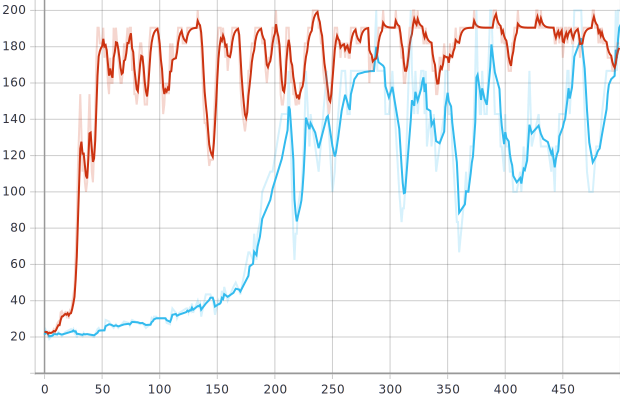
\includegraphics[width=0.55\columnwidth]{images/ep-ret-mean.png}
  \caption{Mean episodic return of the two agents. The ANN agent is depicted in
    red, while the SNN agent is depicted in blue. The ANN agent solves the task
    quicker than the SNN.\label{fig:ep-ret-mean}}
\end{figure}

Our experimental results (see \autoref{fig:ep-ret-mean}) show that both the ANN
and SNN agents are able to solve the ImageCartpole Environment. The ANN agent is
able to solve the ImageCartPole environment within 50 epochs, while the SNN
agent takes 300 epochs to obtain a solution. However, this suggests that
Reinforcement Learning is still a viable method for learning spiking neural
agents.

\section{Discussion}

The results we obtained demonstrated that spiking neural agents can be directly
trained end-to-end on simple reinforcement learning tasks. While the results
were positive, the current environment setup does not fully exploit the benefit
of spiking neural networks, and it is difficult to motivate the use of spiking
neural networks in this context. At each time-step, observations are converted
to full spike trains. SNNs are often able to make predictions based on early
spikes, albeit less reliable. This is not exploited in the current formulation,
where a full spike train of fixed length is received before an action is taken.

One can imagine a RL environment with the following satisfied:

\begin{enumerate}
  \item The action space should contain a no-op: in the case of the Cartpole
    environment, this is as simple as adding the action of not applying force to
    the cart, instead of choosing between left or right.
  \item At each observation, the observation should be spikes, rather than spike
  trains.
\end{enumerate}

The SNN agent receives spikes at each time-step, and after gaining enough
confidence to take an action, it takes the action at that time-step. SNN agents
may be able to solve such environments by exploiting the temporal information
encoded in the relative timing between spikes. We found it difficult to
reconcile the temporal domain of the spiking neural network, and the RL
environment to define a gradient-based learning algorithm that performs the
appropriate credit-assignment, and hence decided to pause on this front.

\end{document}
